ANUGA version 4.0.1 \citep{anuga} is used: finite volumes on an unstructured triangular mesh, with the DE1 scheme (second-order Runge--Kutta). For a homogeneous mixture of constant density, ANUGA solves the evolution of unit discharge $\mathbf q=h\mathbf u$ through the mass-conservation~\eqref{eq:masa} and momentum-conservation~\eqref{eq:movimiento} equations:
\begin{align}
\partial_t h+\nabla\cdot\mathbf q&=S_h,\label{eq:masa}\\
\partial_t\mathbf q+\nabla\cdot\left(\frac{\mathbf q\otimes\mathbf q}{h}+\tfrac12 gh^2\mathbf I\right)&=-gh\nabla z-\frac{\boldsymbol\tau_b}{\rho_m}+S_h\mathbf u_\mathrm{in},\label{eq:movimiento}
\end{align}
where $h$ is flow thickness (\si{m}); $\mathbf u$, depth-averaged velocity (\si{m.s^{-1}}); $\mathbf q=h\mathbf u$, discharge per unit width (\si{m^2.s^{-1}}); $z$, bed elevation (\si{m}); $g$, gravitational acceleration (\si{m.s^{-2}}); $S_h$, the rate of thickness input (\si{m.s^{-1}}); $\mathbf u_\mathrm{in}$, inflow velocity (\si{m.s^{-1}}); $\boldsymbol\tau_b$, basal shear stress (\si{Pa}); $\rho_m$, mixture density (\si{kg.m^{-3}}); and $\mathbf I$, the identity tensor. After dividing by the constant $\rho_m$, no density factor appears in the pressure or gravity terms. Basal resistance is $\boldsymbol\tau_b/\rho_m=ghS_f\,\mathbf u/U$, with $U=|\mathbf u|$ and friction slope $S_f$ given by
\begin{equation}
S_f=\frac{\tau_y}{\rho_m g h}+\frac{K\eta U}{8\rho_m g h^2}+\frac{n_\mathrm{td}^2U^2}{h^{4/3}},\label{eq:friccion}
\end{equation}
where $\tau_y$ is yield stress (\si{Pa}); $\eta$, the dynamic viscosity of the mixture (\si{Pa.s}); $K$, the dimensionless laminar resistance parameter; and $n_\mathrm{td}$, the equivalent Manning coefficient for turbulence and dispersion (\si{s.m^{-1/3}}). Yield stress and viscosity are obtained from the rheological relationships
\begin{equation}
\tau_y=0.1\,\alpha_2e^{\beta_2\Cvf},\qquad \eta=0.1\,\alpha_1e^{\beta_1\Cvf},\label{eq:reologia}
\end{equation}
where $\Cvf$ is the volumetric concentration of the fine matrix; in contrast, density $\rho_m$ uses the total concentration $\Cvt$ (Section~\ref{sec:marco}). The sweep simulations adopt $\Cvt=\Cvf$. The coefficients $(\alpha_1,\beta_1,\alpha_2,\beta_2)$ come from Table~13 of \citet{flo2d2021}, where $\alpha_1$ is expressed in poise and $\alpha_2$ in \si{dyn.cm^{-2}}; $\beta_1$ and $\beta_2$ are dimensionless. The factor 0.1 in~\eqref{eq:reologia} converts both quantities to SI units, so that $\tau_y$ is in \si{Pa} and $\eta$ in \si{Pa.s}. The Glenwood~2 sample appears in three variants in different versions of the documentation and was treated as a sensitivity test. $K$ and $n_\mathrm{td}$ vary by surface: on paved streets $K=100$ and $n_\mathrm{td}=0.025$; elsewhere, $K=400$ and $n_\mathrm{td}=0.050$.

Resistance~\eqref{eq:friccion} is applied as a fractional step and solved implicitly in each cell. With $a=\tau_y/(\rho_m h)$, $b=K\eta/(8\rho_m h^2)$, $c=gn_\mathrm{td}^2/h^{4/3}$ and $r=(U^*-\Delta t\,a)_+$, the result is
\begin{equation}
U^{n+1}=\frac{2r}{1+b\Delta t+\sqrt{(1+b\Delta t)^2+4c\Delta t\,r}},\label{eq:resistencia}
\end{equation}
where the asterisk indicates the state before the resistance step; the superscript $n+1$, the state after that step; $\Delta t$ is the time step and $(x)_+=\max(x,0)$. Solution~\eqref{eq:resistencia} satisfies $0\le U^{n+1}\le U^*$, preserves direction, dissipates energy and does not modify $h$. If $|\mathbf q^*|\le\Delta t\,\tau_y/\rho_m$, the cell stops and may reactivate in subsequent steps. ANUGA's own Manning friction is set to zero to avoid duplicating resistance.

The mixture enters through a triangular hydrograph with peak discharge $Q_p$, mixture volume $V_m$ and time to peak of \SI{600}{s}, with base $T_B=2V_m/Q_p$. In a circle of radius \SI{14}{m}, each source adds the thickness increment $\Delta h$ corresponding to the volume supplied by the hydrograph during the step, together with its momentum: $h^+=h^-+\Delta h$ and $\mathbf q^+=\mathbf q^-+\Delta h\,\mathbf u_\mathrm{in}$, where superscripts $-$ and $+$ indicate the states before and after the input, and $\mathbf u_\mathrm{in}$ is oriented along the channel axis. When $Q=0$, there is no forcing. In H3, each source receives the fraction of the hydrograph corresponding to its catchment area. The first-generation mesh has about \num{4.3e5} triangles: \SI{40}{m^2} in the corridor between the channels and Padre Hurtado (equivalent side length of about \SI{10}{m}) and \SI{600}{m^2} outside it. Gravitational acceleration is $g=\SI{9.8}{m.s^{-2}}$ throughout the model. In the first generation, simulations last $T_B+\SI{1200}{s}$, and the volume balance is recorded in each. The city, measured-rainfall and fine-campus-mesh variants are described in Sections~\ref{sec:res-v4} and~\ref{sec:res-posterior}.

\begin{table}[htbp]\centering\small
\caption{Physical and numerical parameters applied in the simulations. Rheological coefficients are from the O'Brien and Julien sample table compiled in the FLO-2D manual \citep{flo2d2021}; $\tau_y=0.1\,\alpha_2e^{\beta_2C_v}$ in Pa and $\eta=0.1\,\alpha_1e^{\beta_1C_v}$ in Pa\,s.}\label{tab:parametros}
\begin{adjustbox}{max width=\textwidth}\begin{tabular}{lrrrrrrr}\toprule
Sample & $\alpha_1$ & $\beta_1$ & $\alpha_2$ & $\beta_2$ & \multicolumn{3}{c}{$\tau_y$ (Pa) / $\eta$ (Pa\,s) with $C_v=$}\\\cmidrule(l){6-8}
 & & & & & 0.35 & 0.40 & 0.45\\\midrule
Glenwood 1 & 0.0028 & 23.00 & 0.0345 & 20.10 & 3.9 / 0.89 & 10.7 / 2.80 & 29.2 / 8.85\\
Glenwood 2a & 0.0648 & 6.20 & 0.0765 & 16.90 & 2.8 / 0.06 & 6.6 / 0.08 & 15.4 / 0.11\\
Glenwood 2b & 0.6480 & 6.20 & 0.0765 & 16.90 & 2.8 / 0.57 & 6.6 / 0.77 & 15.4 / 1.06\\
Glenwood 2c & 0.6480 & 8.20 & 0.0765 & 16.90 & 2.8 / 1.14 & 6.6 / 1.72 & 15.4 / 2.59\\
Aspen 1 & 0.0360 & 22.10 & 0.1810 & 25.70 & 145.9 / 8.23 & 527.5 / 24.86 & 1,906.8 / 75.05\\
Aspen 2 & 0.0538 & 14.50 & 2.7200 & 10.40 & 10.4 / 0.86 & 17.4 / 1.78 & 29.3 / 3.67\\
\midrule
\multicolumn{8}{l}{\textbf{Mixture and constants}}\\
\multicolumn{5}{l}{Water density $\rho_w$ / solids density $\rho_s$} & \multicolumn{3}{r}{\SI{1000}{kg/m^3} / \SI{2650}{kg/m^3}}\\
\multicolumn{5}{l}{Mixture density $\rho_m=\rho_w+C_v(\rho_s-\rho_w)$, $C_v=0.35/0.40/0.45$} & \multicolumn{3}{r}{1,578 / 1,660 / 1,742 kg/m$^3$}\\
\multicolumn{5}{l}{Gravity $g$} & \multicolumn{3}{r}{\SI{9.8}{m/s^2}}\\
\multicolumn{5}{l}{Laminar resistance $K$ (streets / elsewhere)} & \multicolumn{3}{r}{100 / 400}\\
\multicolumn{5}{l}{Turbulent-dispersive Manning $n_{td}$ (streets / elsewhere)} & \multicolumn{3}{r}{0.025 / 0.050 s\,m$^{-1/3}$}\\
\multicolumn{8}{l}{\textbf{Input, mesh and computation}}\\
\multicolumn{5}{l}{Mixture volume $V$ / peak discharge $Q_p$ / time to peak $t_p$} & \multicolumn{3}{r}{80--300 thousand m$^3$ / 100--250 m$^3$/s / 600 s}\\
\multicolumn{5}{l}{Inflow velocity / radius of each source} & \multicolumn{3}{r}{2 m/s / 14 m}\\
\multicolumn{5}{l}{Maximum triangle area (corridor / elsewhere); triangles, first model generation} & \multicolumn{3}{r}{40 / 600 m$^2$; $\approx$430,000}\\
\multicolumn{5}{l}{Terrain grid; street lowering; assumed building height} & \multicolumn{3}{r}{4 m; 0.15 m; 6 m}\\
\multicolumn{5}{l}{Courant number (screening / rainfall / final)} & \multicolumn{3}{r}{1 / 0.5 / $\le$0.25}\\
\multicolumn{5}{l}{Wetting threshold for evaluation $h^*$} & \multicolumn{3}{r}{5 cm (sensitivity 2 and 10 cm)}\\
\bottomrule\end{tabular}\end{adjustbox}\end{table}

\begin{figure}[htbp]\centering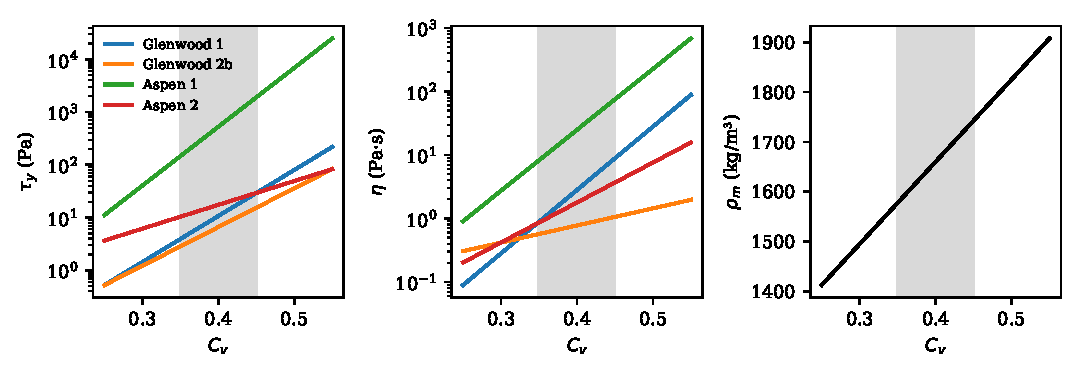
\includegraphics[width=\textwidth]{reologia}\caption{Calculated mixture properties as a function of volumetric solids concentration $C_v$ for the samples tested: yield stress $\tau_y$, viscosity $\eta$ and density $\rho_m$. The gray band indicates the initial range (0.35--0.45); subsequent tests extend the concentrations (Section~\ref{sec:res-posterior}).}\label{fig:reologia}\end{figure}
